\documentclass[]{scrartcl}
\usepackage{lmodern}
\usepackage{amssymb,amsmath}
\usepackage{ifxetex,ifluatex}
\usepackage{fixltx2e} % provides \textsubscript
\ifnum 0\ifxetex 1\fi\ifluatex 1\fi=0 % if pdftex
  \usepackage[T1]{fontenc}
  \usepackage[utf8]{inputenc}
\else % if luatex or xelatex
  \ifxetex
    \usepackage{mathspec}
  \else
    \usepackage{fontspec}
  \fi
  \defaultfontfeatures{Ligatures=TeX,Scale=MatchLowercase}
\fi
% use upquote if available, for straight quotes in verbatim environments
\IfFileExists{upquote.sty}{\usepackage{upquote}}{}
% use microtype if available
\IfFileExists{microtype.sty}{%
\usepackage{microtype}
\UseMicrotypeSet[protrusion]{basicmath} % disable protrusion for tt fonts
}{}
\usepackage{hyperref}
\hypersetup{unicode=true,
            pdftitle={Angabe},
            pdfauthor={Team\ldots{}},
            pdfborder={0 0 0},
            breaklinks=true}
\urlstyle{same}  % don't use monospace font for urls
\IfFileExists{parskip.sty}{%
\usepackage{parskip}
}{% else
\setlength{\parindent}{0pt}
\setlength{\parskip}{6pt plus 2pt minus 1pt}
}
\setlength{\emergencystretch}{3em}  % prevent overfull lines
\providecommand{\tightlist}{%
  \setlength{\itemsep}{0pt}\setlength{\parskip}{0pt}}
\setcounter{secnumdepth}{5}
% Redefines (sub)paragraphs to behave more like sections
\ifx\paragraph\undefined\else
\let\oldparagraph\paragraph
\renewcommand{\paragraph}[1]{\oldparagraph{#1}\mbox{}}
\fi
\ifx\subparagraph\undefined\else
\let\oldsubparagraph\subparagraph
\renewcommand{\subparagraph}[1]{\oldsubparagraph{#1}\mbox{}}
\fi

\usepackage{graphicx}
\usepackage{array}
\usepackage{ragged2e}
\usepackage[section]{placeins}
\makeatletter
\AtBeginDocument{%
  \expandafter\renewcommand\expandafter\subsection\expandafter{%
    \expandafter\@fb@secFB\subsection
  }%
}
\makeatother
 
\title{Angabe 1}
\providecommand{\subtitle}[1]{}
\subtitle{Untertitel}
\author{Daniel Graf, Dimitrie Diez, Arne Schöntag, Peter Müller}
\date{}

\begin{document}
\maketitle


\tableofcontents

\section{Einführung}

% Problem -> Motivation

\section{Messexperiment}

Das Messexperiment wurde am $05.04.2017$ im Lichthof der Hochschule München (Lothstraße 64) durchgeführt. Es nahmen $22$ Probanden im Alter von $20-29$ Jahren teil. Das Experiment bestand aus drei Teilen. 

Zunächst wurde die Wunschgeschwindigkeit in der Ebene gemessen. Hierfür ging jeder Proband eine markierte Strecke von $27,3m$ ab und stoppte die hierfür benötigte Zeit. Anschließend wurde dieser Vorgang zweimal wiederholt und die entsprechende Rundennummer vermerkt. Im zweiten Teil erfolgte die Messung der benötigten Zeit für einen Treppenaufstieg. Die Treppenlänge betrug $9m$. Jeder Proband führte den Vorgang dreimal durch und vermerkte die benötigte Zeit und die entsprechende Rundennummer. Analog hierzu wurde im dritten Teil des Experiments die Zeit beim Treppenabstieg gemessen. 

Neben den gemessenen Zeiten in jeder Runde, dem Alter und der Körpergröße ist auch das Geschlecht jedes Probanden bekannt. Weitere Informationen sind in der beiliegenden Versuchsbeschreibung "Choreographie\_Treppengeschwindigkeit\_2017" aufgeführt. In den folgenden Kapiteln erfolgt die Auswertung der ermittelten Messwerte.

\section{Überprüfung auf Normalverteilung}

Um zu überprüfen, ob die erhobenen Daten normalverteilt sind, kann eine Vielzahl verschiedener Methoden angewandt werden. Für eine aussagekräftige Beurteilung beschränkt sich diese Arbeit auf zwei grafische und drei rechnerische Methoden. Als grafische Verfahren werden ein Histogramm und ein Quantil-Quantil-Diagramm erstellt. Im Anschluss erfolgt die rechnerische Überprüfung mittels Shapiro-Wilk-, Cramér-von-Mises- und Anderson-Darling-Test. Aus den gemessenen Zeiten werden die Geschwindigkeiten der einzelnen Probanden ermittelt und für die erwähnten Testverfahren herangezogen. Die Geschwindigkeiten in der Ebene, beim Treppenaufstieg sowie beim Treppenabstieg werden jeweils gesondert betrachtet.

\subsection{In der Ebene}
Vor der Analyse muss geprüft werden, ob alle Daten plausibel sind, oder ob bestimmte Daten von der Analyse ausgeschlossen werden müssen. Bei der Betrachtung der einzelnen Messergebnisse fällt auf, dass ein Proband deutlich langsamer als die restlichen Probanden gegangen ist. Trotz dessen werden alle Messdaten berücksichtigt, da anzunehmen ist, dass es immer Personen gibt, die langsamer oder schneller als die Mehrheit gehen. Es ist jedoch anzumerken, dass bei einem Versuch mit nur einer geringen Anzahl von Probanden, solche Ausreißer eventuell eine signifikante Abweichung verursachen.

\subsubsection{Grafische Überprüfung}
In Abbildung \ref{fig:histogramm_ebene} wird die Verteilung der Geschwindigkeiten einer Normalverteilungskurve gegenübergestellt. Für die Berechnung der Normalverteilungskurve wurden Erwartungswert und Standardabweichung der Ergebnisse ermittelt. Der Erwartungswert beträgt $1,48\ \frac{m}{s}$ und die Standardabweichung $0,144\ \frac{m}{s}$. Das Histogramm bildet relative Häufigkeiten ab. Es fällt auf, dass eine deutliche Häufung der Ergebnisse in den Bereich des Maximums der Normalverteilungskurve fällt. Dies ist ein Anzeichen für eine Normalverteilung der Ergebnisse. Allerdings befinden sich auch an den Rändern der Normalverteilungskurve noch kleinere Häufungen der Ergebnisse. Somit kann aus dem Histogramm kein eindeutiger Rückschluss auf eine Normalverteilung der Geschwindigkeiten gezogen werden. Grundsätzlich ist die Darstellung des Histogramms stark von der gewählten Anzahl an Klassen abhängig und ist gerade bei kleineren Messreihen nicht aussagekräftig.
\begin{figure}[htpb]
\centering
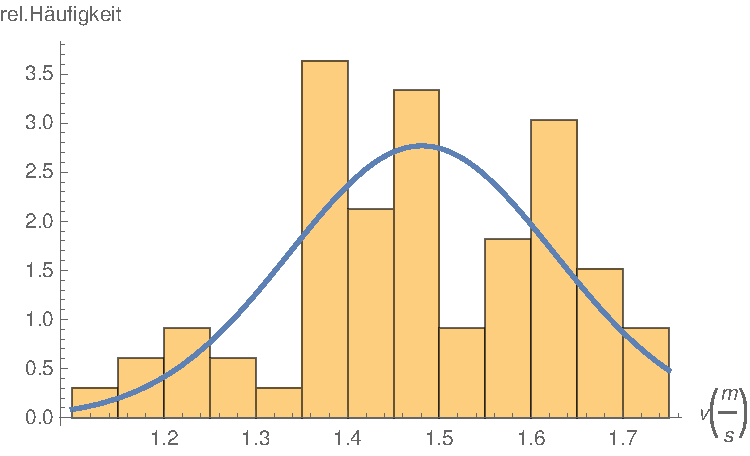
\includegraphics[width=0.8\textwidth]{abbildungen/Histogramm_2017_Ebene.pdf}
\caption{Histogramm der Geschwindigkeiten in der Ebene im Vergleich zur Normalverteilung}
\label{fig:histogramm_ebene}
\end{figure}

Abbildung \ref{fig:qqplot_ebene} veranschaulicht die Verteilung der Geschwindigkeiten in einem Quantil-Quantil Diagramm. In diesem Diagramm sind die gemessenen Geschwindigkeiten gegenüber der Normalverteilung abgebildet. Da sich die Mehrheit der geplotteten Punkte auf oder in unmittelbarer Nähe der Diagonalen befindet, spricht dieses Diagramm für eine Normalverteilung der Geschwindigkeiten. Für eine aussagekräftigere Beurteilung wird diese Thematik im Folgenden mit rechnerischen Tests überprüft.
\begin{figure}[htpb]
\centering
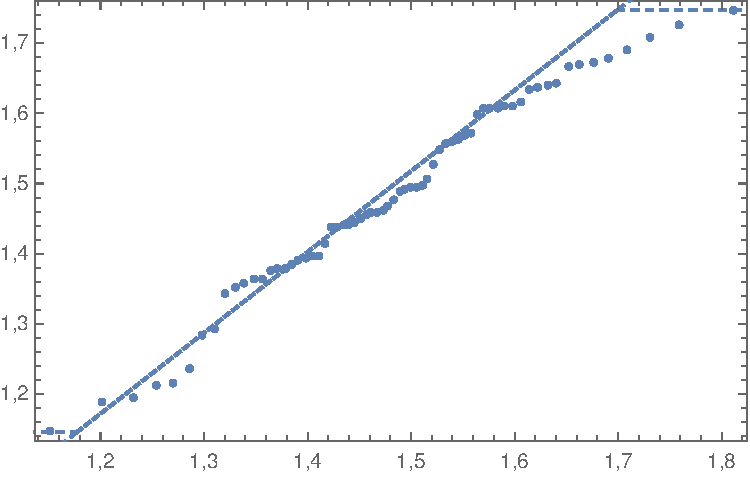
\includegraphics[width=0.7\textwidth]{abbildungen/QQ_Plot_2017_Ebene.pdf}
\caption{Quantil-Quantil-Diagramm der Geschwindigkeiten in der Ebene in $\frac{m}{s}$}
\label{fig:qqplot_ebene}
\end{figure}

\subsubsection{Rechnerische Überprüfung}

Tabelle \ref{tab:anpassungstest_ebene} zeigt die Ergebnisse von mehreren Anpassungstests. Dabei werden die Messdaten auf Normalverteilung getestet. Exemplarisch werden im Folgenden Shapiro-Wilk-, Cramér-von-Mises- und Anderson-Darling-Test näher betrachtet und analysiert.  

Laut dem Shapiro-Wilk-Test wird die Nullhypothese "Die Geschwindigkeiten sind normalverteilt" nicht verworfen, da der P-Wert das Signifikanzniveau von $0,05$ überschreitet. Auch der Cramér-von-Mises-Test ergibt einen P-Wert von $0,84$ und ist somit ebenfalls deutlich über dem Signifikanzniveau. Analog hierzu liefert der Anderson-Darling-Test einen weiteren Nachweis für die Normalverteilung der Geschwindigkeiten, da der P-Wert von $0,82$ die $0,05$ des Signifikanzniveaus ebenfalls überschreitet. (Der Anderson-Darling-Test gilt als aussagekräftigster statistischer Test)

Betrachtet man abschließend alle ermittelten Ergebnisse, kann man davon ausgehen, dass die Geschwindigkeiten der Probanden in der Ebene normalverteilt sind. 
\begin{table}
\centering
\begin{tabular}{l|ll}
 \text{} & \text{Statistic} & \text{P-Value} \\
\hline
 \text{Anderson-Darling} & 0.426988 & 0.821001 \\
 \text{Baringhaus-Henze} & 0.269634 & 0.785711 \\
 \text{Cram{\' e}r-von Mises} & 0.0560719 & 0.838694 \\
 \text{Jarque-Bera ALM} & 1.57313 & 0.376383 \\
 \text{Mardia Combined} & 1.57313 & 0.376383 \\
 \text{Mardia Kurtosis} & -0.879486 & 0.379138 \\
 \text{Mardia Skewness} & 0.82605 & 0.363417 \\
 \text{Pearson }$\chi ^2$ & 14.6667 & 0.144695 \\
 \text{Shapiro-Wilk} & 0.975506 & 0.215767 \\
\end{tabular}
\caption{Anpassungstests zur Überprüfung der gemessenen Geschwindigkeiten in der Ebene auf Normalverteilung}
\label{tab:anpassungstest_ebene}
\end{table}



\subsection{Beim Treppenaufstieg}
\subsubsection{Grafische Überprüfung}
Bei der Betrachtung der Messergebnisse für den Treppenaufstieg fällt auf, dass vier Probanden stets mit höherer Geschwindigkeit gehen als die restlichen Probanden. Dieses Verhalten wiederholt sich über alle Runden. Aufgrund der geringen Anzahl an Messwerten fällt dies bei der Auswertung stark ins Gewicht. 

Für die weitere Überprüfung auf Normalverteilung werden zwei Auswertungen durchgeführt. Eine Auswertung erfolgt über alle Messreihen hinweg. Die betroffenen Probanden haben beim Aufstieg immer mehrere Treppen übersprungen. Es ist nicht auszuschließen, dass es in der Bevölkerung einen Anteil von Menschen gibt, die dieses Verhalten grundsätzlich aufweisen. Anschließend wird eine Auswertung durchgeführt, bei welcher die Ausreißer ausgeschlossen werden, da die Möglichkeit besteht, dass es sich um eine Anomalie oder um Sabotage handelt. 

\begin{figure}[!htb]
    \centering
    \begin{minipage}{.5\textwidth}
        \centering
        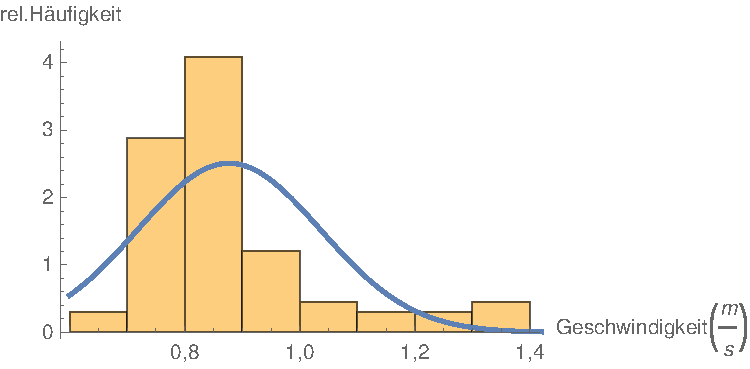
\includegraphics[width=\textwidth]{abbildungen/Histogramm_2017_TreppeAuf_MitAusreisser.pdf}
        \caption{Histogramm der Geschwindig-keiten beim Treppenaufstieg mit Ausreißern im Vergleich zur Normalverteilung}
        \label{fig:Histogramm_TreppeAuf_MA}
    \end{minipage}%
    \begin{minipage}{0.5\textwidth}
        \centering
        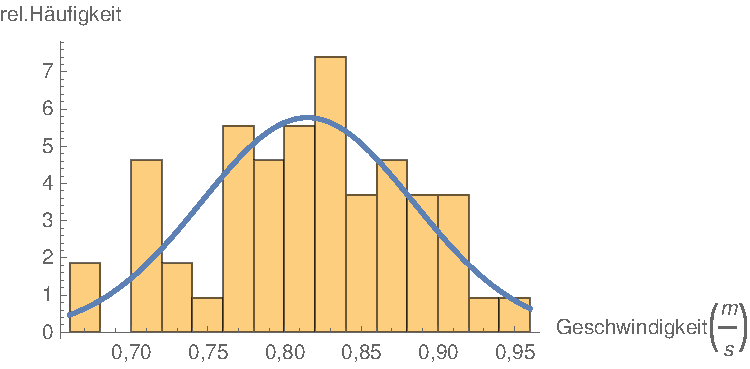
\includegraphics[width=\textwidth]{abbildungen/Histogramm_2017_TreppeAuf_OhneAusreisser.pdf}
        \caption{Histogramm der Geschwindig-keiten beim Treppenaufstieg ohne Ausreißer im Vergleich zur Normalverteilung}
        \label{fig:Histogramm_TreppeAuf_OA}
    \end{minipage}
\end{figure}

Das Histogramm in der Abbildung \ref{fig:Histogramm_TreppeAuf_MA} deutet auf eine rechtsschiefe Verteilung der Geschwindigkeiten hin. Dies stellt ein Indiz gegen eine Normalverteilung der Messwerte dar. Im Gegensatz dazu weist das Histogramm in Abbildung \ref{fig:Histogramm_TreppeAuf_OA} eine symmetrische Verteilung auf. Daher ist anzunehmen, dass die Messwerte ohne Ausreißer normalverteilt sind. Aber wie bereits erwähnt, sind Histogramme nur bedingt aussagekräftig. Eine genauere grafische Betrachtung erfolgt über ein Quantil-Quantil-Diagramm.

In Abbildung \ref{fig:QQ_TreppeAuf_MA} ist deutlich eine Abweichung von der Normalverteilung zu sehen, da einige Werte weit von der Diagonalen entfernt sind. Dies ist auf die erwähnten vier Probanden zurückzuführen. Im Gegensatz dazu deutet die Abbildung \ref{fig:QQ_TreppeAuf_OA} auf eine Normalverteilung hin, da alle Quantile auf oder in unmittelbarer Nähe der Diagonalen liegen.
\begin{figure}[!htb]
    \centering
    \begin{minipage}{.5\textwidth}
        \centering
        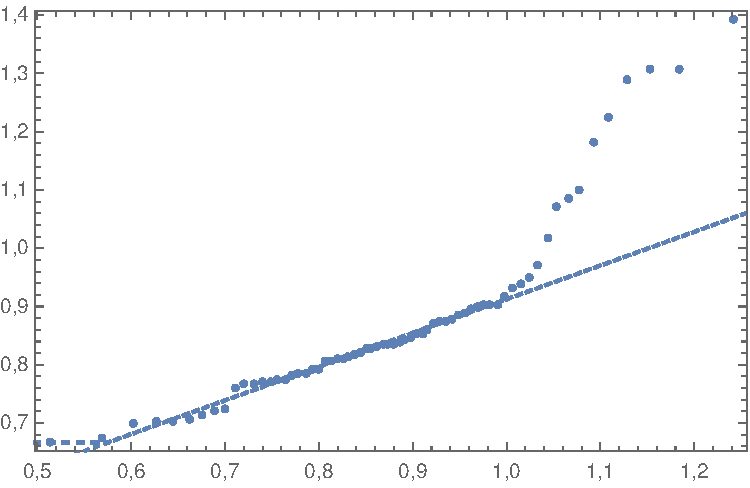
\includegraphics[width=\textwidth]{abbildungen/QQ_Plot_2017_TreppeAuf_MitAusreisser.pdf}
        \caption{Quantil-Quantil-Diagramm der Geschwindigkeiten beim Treppenaufstieg mit Ausreißern in $\frac{m}{s}$}
        \label{fig:QQ_TreppeAuf_MA}
    \end{minipage}%
    \begin{minipage}{0.5\textwidth}
        \centering
        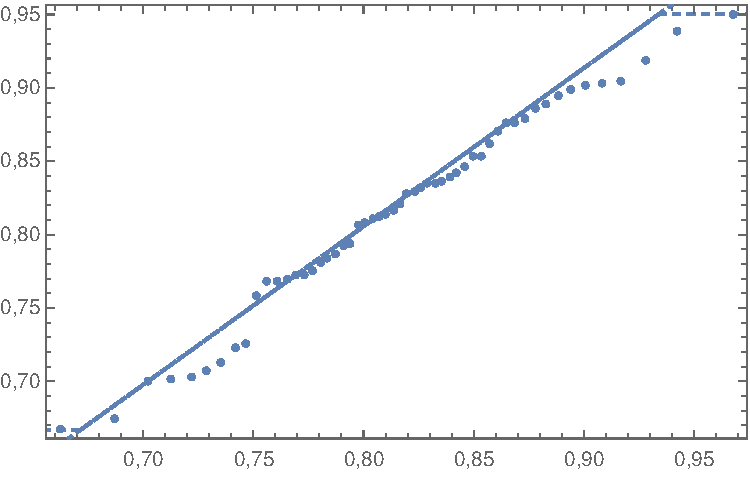
\includegraphics[width=\textwidth]{abbildungen/QQ_Plot_2017_TreppeAuf_OhneAusreisser.pdf}
        \caption{Quantil-Quantil-Diagramm der Geschwindigkeiten beim Treppenaufstieg ohne Ausreißer in $\frac{m}{s}$}
        \label{fig:QQ_TreppeAuf_OA}
    \end{minipage}
\end{figure}


\subsubsection{Rechnerische Überprüfung}
Die Anpassungstests zeigen, dass die Geschwindigkeiten bei einem Treppenaufstieg nicht normalverteilt sind, wenn man die Ausreißer mitberücksichtigt. Die Tabelle \ref{tab:anpassungstest_TreppeAuf_MA} zeigt, dass bei einem Cram{\' e}r-von Mises Test ein p-Wert von nur $0,018$ erreicht wird, welcher somit deutlich geringer als das Signifikanzniveau von $0,05$ ist. Werden die Ausreißer nicht mitberücksichtigt, so ergibt der Cram{\' e}r-von Mises Test einen p-Wert von $0,92$, wie in Tabelle \ref{tab:anpassungstest_TreppeAuf_OA} zu sehen. Auch der Anderson-Darling Test liegt weit über dem Signifikanzniveau. Die rechnerische Überprüfung bestätigt somit das Ergebnis der grafischen Analyse. Wie bereits erwähnt, sind die Ausreißer immer von denselben vier Probanden verursacht worden. Diese haben beim Aufsteigen der Treppen in jeder Runde mehrere Stufen übersprungen. Die Vermutung liegt nahe, dass es eine Gruppe von Menschen gibt, die beim Aufsteigen der Treppen grundsätzlich schneller gehen. Eine genaue Untersuchung ist mit einer deutlich größeren Anzahl der Probanden notwendig.
\begin{table}
    \centering
    \begin{minipage}{.47\textwidth}
\centering
\begin{tabular}{l|ll}
 \text{} & \text{Statistic} & \text{P-Value} \\
\hline
 \text{Anderson-Darling} & 0.33829 & 0.90645 \\
 \text{Baringhaus-Henze} & 0.213705 & 0.858651 \\
 \text{Cram{\' e}r-von Mises} & 0.0421682 & 0.921661 \\
 \text{Jarque-Bera ALM} & 1.31475 & 0.440072 \\
 \text{Mardia Combined} & 1.31475 & 0.440072 \\
 \text{Mardia Kurtosis} & -0.891517 & 0.372652 \\
 \text{Mardia Skewness} & 0.553342 & 0.456956 \\
 \text{Pearson }$\chi ^2$ & 12.2963 & 0.197116 \\
 \text{Shapiro-Wilk} & 0.977864 & 0.414303 \\
\end{tabular}
\caption{Anpassungstests zur Überprüfung der gemessenen Geschwindigkeiten beim Treppenaufstieg ohne Ausreissern auf Normalverteilung}
\label{tab:anpassungstest_TreppeAuf_OA}
    \end{minipage}%
    \begin{minipage}{0.06\textwidth}
     \hfill
    \end{minipage}%
    \begin{minipage}{0.47\textwidth}
\centering
\begin{tabular}{l|ll}
 \text{} & \text{Statistic} & \text{P-Value} \\
\hline
 \text{Anderson-Darling} & 3.67396 & 0.0126832 \\
 \text{Baringhaus-Henze} & 4.53865 & 0.000403182 \\
 \text{Cram{\' e}r-von Mises} & 0.638786 & 0.0179638 \\
 \text{Jarque-Bera ALM} & 45.2212 & 0.000864057 \\
 \text{Mardia Combined} & 45.2212 & 0.000864057 \\
 \text{Mardia Kurtosis} & 3.44345 & 0.000574336 \\
 \text{Mardia Skewness} & 26.5574 & \text{2.55817*$10^{-7}$} \\
 \text{Pearson }$\chi ^2$ & 25. & 0.00534551 \\
 \text{Shapiro-Wilk} & 0.835009 & \text{4.31299*$10^{-7}$} \\
\end{tabular}
\caption{Anpassungstests zur Überprüfung der gemessenen Geschwindigkeiten beim Treppenaufstieg mit Ausreissern auf Normalverteilung}
\label{tab:anpassungstest_TreppeAuf_MA}
    \end{minipage}
\end{table}

\subsection{Beim Treppenabstieg}

Bei der Messung zum Abstieg von der Treppe gibt es wenig besondere Fälle. Die gemessenen Daten weisen nur wenige unregelmäßige Ausreißer aus. Diese werden erwartungsgemäß geringen Einfluss haben. Beim Treppenaufstieg wurden signifikante Unterschiede durch 
die Ausreißer festgestellt. Deswegen werden analog zum Aufstieg beim Abstieg auch zwei Analysen durchgeführt.



\subsubsection{Grafische Überprüfung}
Ein Vergleich der Histogramme in den Abbildungen \ref{fig:Histogramm_TreppeAb_MA} und \ref{fig:Histogramm_TreppeAb_OA} zeigt, dass die Ausreißer nur einen geringen Unterschied verursachen. In den Abbildungen ist jeweils eine Normalverteilungskurve dargestellt. Es zeigt sich, dass eine Normalverteilung nicht genau erkennbar ist.

Beim Betrachten des Quantil-Quantil-Diagramms in Abbildung \ref{fig:QQ_TreppeAb_MA} und \ref{fig:QQ_TreppeAb_OA}, zeigt sich ebenfalls, dass der Unterschied der gesamten Daten und der bereinigten Daten sehr gering und mit bloßem Auge nicht zu erkennen ist. Aus den beiden Diagrammen wird deutlich, dass es sich bei beiden Fällen um eine Normalverteilung handelt, da der P-Wert in beiden Fällen über dem Signifikanzniveau von $0,05$ liegt.

\begin{figure}[!htb]
    \centering
    \begin{minipage}{.49\textwidth}
        \centering
        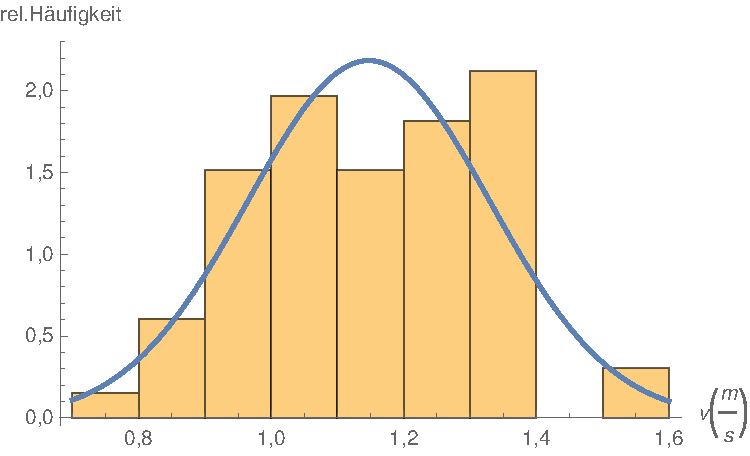
\includegraphics[width=\textwidth]{abbildungen/Histogramm_2017_TreppeAb_MitAusreisser.pdf}
        \caption{Histogramm der Geschwindig-keiten beim Treppenabstieg mit Ausreißern im Vergleich zur Normalverteilung}
        \label{fig:Histogramm_TreppeAb_MA}
    \end{minipage}%
    \begin{minipage}{0.02\textwidth}
     \hfill
    \end{minipage}%
    \begin{minipage}{0.49\textwidth}
        \centering
        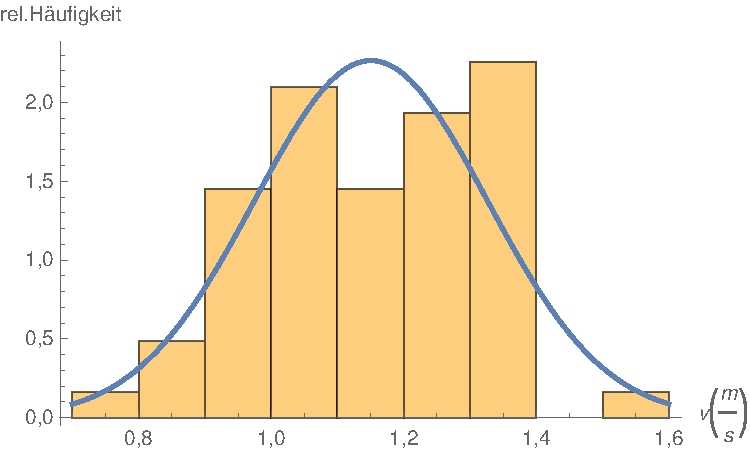
\includegraphics[width=\textwidth]{abbildungen/Histogramm_2017_TreppeAb_OhneAusreisser.pdf}
        \caption{Histogramm der Geschwindig-keiten beim Treppenabstieg ohne Ausreißer im Vergleich zur Normalverteilung}
        \label{fig:Histogramm_TreppeAb_OA}
    \end{minipage}
\end{figure}


\begin{figure}[!htb]
    \centering
    \begin{minipage}{.49\textwidth}
        \centering
        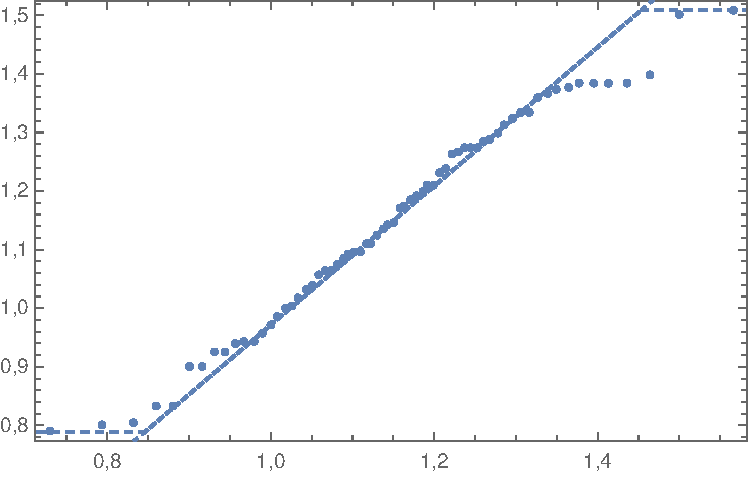
\includegraphics[width=\textwidth]{abbildungen/QQ_Plot_2017_TreppeAb_MitAusreisser.pdf}
        \caption{Quantil-Quantil-Diagramm der Geschwindigkeiten beim Treppenabstieg mit Ausreißern in $\frac{m}{s}$}
        \label{fig:QQ_TreppeAb_MA}
    \end{minipage}%
    \begin{minipage}{0.02\textwidth}
     \hfill
    \end{minipage}%
    \begin{minipage}{0.49\textwidth}
        \centering
        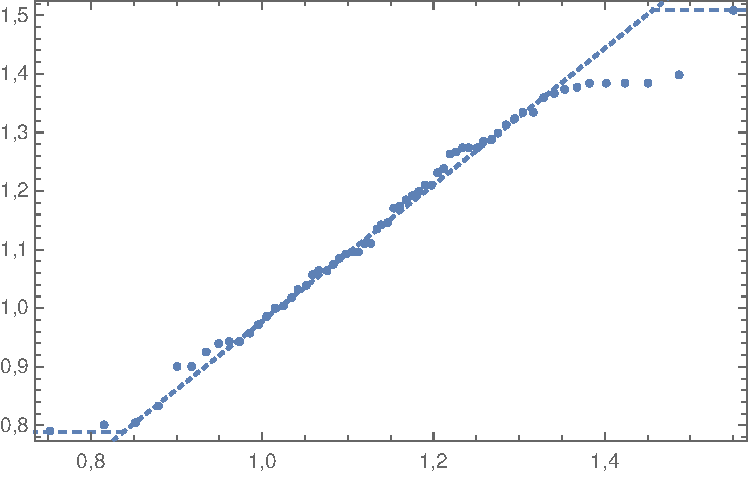
\includegraphics[width=\textwidth]{abbildungen/QQ_Plot_2017_TreppeAb_OhneAusreisser.pdf}
        \caption{Quantil-Quantil-Diagramm der Geschwindigkeiten beim Treppenabstieg ohne Ausreißer in $\frac{m}{s}$}
        \label{fig:QQ_TreppeAb_OA}
    \end{minipage}
\end{figure}




\subsection{Rechnerische Überprüfung}
Die rechnerische Überprüfung bestätigt die Analyse des Quantil-Quantil-Diagramms. Wie in Tabelle \ref{tab:anpassungstest_TreppeAb_MA} und Tabelle \ref{tab:anpassungstest_TreppeAbf_OA} zu sehen, liegt in beiden Fällen eine Normalverteilung vor. Es ist zu bemerken, dass ein Anpassungstest anhand der Daten mit Ausreißern einen größeren p-Wert erzielt. 
\begin{table}
    \centering
    \begin{minipage}{.47\textwidth}
\centering
\begin{tabular}{l|ll}
  \text{} & \text{Statistic} & \text{P-Value} \\
\hline
 \text{Anderson-Darling} & 0.440903 & 0.806782 \\
 \text{Baringhaus-Henze} & 0.420106 & 0.556077 \\
 \text{Cram{\' e}r-von Mises} & 0.0609776 & 0.807822 \\
 \text{Jarque-Bera ALM} & 2.23559 & 0.247476 \\
 \text{Mardia Combined} & 2.23559 & 0.247476 \\
 \text{Mardia Kurtosis} & -1.43247 & 0.152009 \\
 \text{Mardia Skewness} & 0.156589 & 0.692316 \\
 \text{Pearson }$\chi ^2$ & 10.3333 & 0.411752 \\
 \text{Shapiro-Wilk} & 0.974316 & 0.186898 \\
\end{tabular}
\caption{Anpassungstests zur Überprüfung der gemessenen Geschwindigkeiten beim Treppenabstieg mit Ausreissern auf Normalverteilung}
\label{tab:anpassungstest_TreppeAb_MA}
    \end{minipage}%
    \begin{minipage}{0.06\textwidth}
     \hfill
    \end{minipage}%
    \begin{minipage}{0.47\textwidth}
\centering
\begin{tabular}{l|ll}
 \text{} & \text{Statistic} & \text{P-Value} \\
\hline
 \text{Anderson-Darling} & 0.54237 & 0.70308 \\
 \text{Baringhaus-Henze} & 0.484286 & 0.455989 \\
 \text{Cram{\' e}r-von Mises} & 0.0788816 & 0.698349 \\
 \text{Jarque-Bera ALM} & 1.99557 & 0.277317 \\
 \text{Mardia Combined} & 1.99557 & 0.277317 \\
 \text{Mardia Kurtosis} & -1.32774 & 0.184265 \\
 \text{Mardia Skewness} & 0.190686 & 0.662346 \\
 \text{Pearson }$\chi ^2$ & 6.37037 & 0.702354 \\
 \text{Shapiro-Wilk} & 0.969539 & 0.183952 \\
\end{tabular}
\caption{Anpassungstests zur Überprüfung der gemessenen Geschwindigkeiten beim Treppenabstieg ohne Ausreissern auf Normalverteilung}
\label{tab:anpassungstest_TreppeAbf_OA}
    \end{minipage}
\end{table}

\section{Modell}



\section{Lineare Regression 2017}

Um Hinweise auf einen möglichen Zusammenhang der Treppengeschwindigkeit mit weiteren durch das Messexperiment ermittelten Größen zu finden, wird eine lineare 
Regression angewandt.

Die hier betrachteten Größen sind Wunschgeschwindigkeit (in der Ebene),
Körpergröße und Rundennummer. Es wird gesondert die Treppengeschwindigkeit aufwärts und abwärts betrachtet.
Zunächst wird nur auf eine Abhängigkeit überprüft, danach die Abhängigkeit von mehreren kombinierten Größen. Die Zusammenhänge werden bezüglich ihrer Plausibilität bewertet.

\subsection{Prüfung auf eine einfache Abhängigkeit}

Hier werden sechs Gleichungen mittels linearer Regression ermittelt: 

\[v_{auf}(v_{ebene}) = \beta_0 + \beta_1 v_{ebene}\]
\[v_{ab}(v_{ebene}) = \beta_0 + \beta_1 v_{ebene}\]

\[v_{auf}(groesse) = \beta_0 + \beta_1 groesse\]
\[v_{ab}(groesse) = \beta_0 + \beta_1 groesse\]

\[v_{auf}(runde) = \beta_0 + \beta_1 runde\]
\[v_{ab}(runde) = \beta_0 + \beta_1 runde\]

\subsubsection{Wunschgeschwindigkeit in der Ebene}

Für die Abhängigkeit Wunschgeschwindigkeit in der Ebene wurde 
der Zusammenhang wie in den Formeln für die Treppengeschwindigkeit aufwärts (\ref{eq:auf2017-ebene}) und abwärts (\ref{eq:ab2017-ebene}) ermittelt. 

\begin{equation} \label{eq:auf2017-ebene}
	v_{auf}(v_{ebene}) = 0.294389 + 0.393467 v_{ebene}
\end{equation}
\begin{equation} \label{eq:ab2017-ebene}
	v_{ab}(v_{ebene}) = 0.475883 + 0.453419 v_{ebene}
\end{equation}

Beide Steigungen sind positiv. Hat ein Proband eine schnellere Wunschgeschwindigkeit in der Ebene, verhält er sich auch schneller auf 
der Treppe. Die Abbildungen \ref{fig:auf2017-ebene} und \ref{fig:ab2017-ebene}
stellen dies grafisch dar. 

\begin{figure} \centering 
	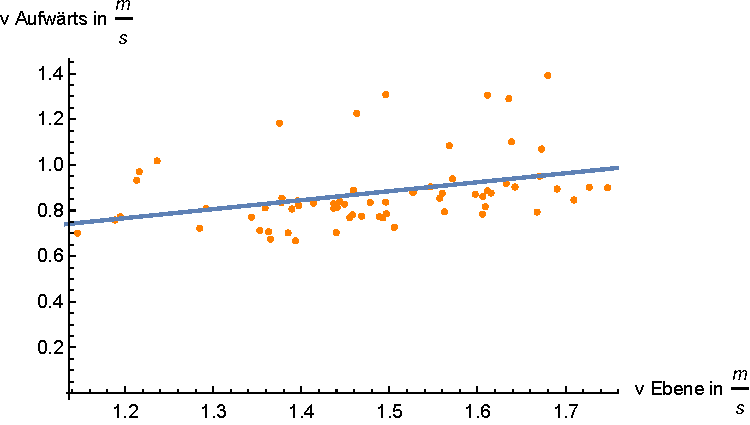
\includegraphics[]{abbildungen/regression/2017/auf-ebene.pdf}
	\[\begin{array}{l|llll}
 \text{} & \text{Estimate} & \text{Standard Error} & \text{t-Statistic} & \text{P-Value} \\
\hline
 1 & 0.506746 & 0.0900029 & 5.63033 & \text{2.603647901106944$\grave{ }$*${}^{\wedge}$-6} \\
 \text{vEbene} & 0.168071 & 0.0588553 & 2.85567 & 0.00727064 \\
\end{array}\]


	\caption{Abhängigkeit Wunschgeschwindigkeit in der Ebene zur Treppengeschwindigkeit aufwärts. Messdaten (orange) mit ermittelter Regressionsgerade (blau). \label{fig:auf2017-ebene}}
\end{figure}

\begin{figure} \centering 
	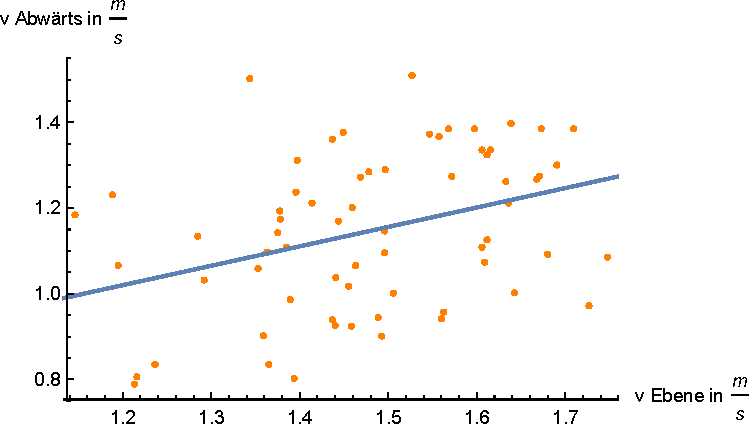
\includegraphics[]{abbildungen/regression/2017/ab-ebene.pdf}
	\[\begin{array}{l|llll}
 \text{} & \text{Estimate} & \text{Standard Error} & \text{t-Statistic} & \text{P-Value} \\
\hline
 1 & 0.440848 & 0.213068 & 2.06904 & 0.0428577 \\
 \text{vEbene} & 0.478525 & 0.142985 & 3.34668 & 0.00141579 \\
\end{array}\]


	\caption{Abhängigkeit Wunschgeschwindigkeit in der Ebene zur Treppengeschwindigkeit abwärts. Messdaten (orange) mit ermittelter Regressionsgerade (blau). \label{fig:ab2017-ebene}}
\end{figure}

In Abbildung \ref{fig:auf2017-ebene} sind wieder
deutlich die schon in der Betrachtung zur Normalverteilung erwähnten Ausreißer zu erkennen. Deshalb wurde die lineare Regression für den gefilterten Messdatensatz (nur Datensätze ohne Bemerkung) durchgeführt. Es ergeben sich neue Formeln für die Treppengeschwindigkeit aufwärts (\ref{eq:ohne-auf2017-ebene}) und abwärts (\ref{eq:ohne-ab2017-ebene}). Dazu gehören Abbildungen \ref{fig:ohne-auf2017-ebene} und \ref{fig:ohne-ab2017-ebene}. Die Ausreißer wurden in der Regression hier nicht verwendet, sind aber hervorgehoben eingezeichnet. Bei der Treppengeschwindigkeit aufwärts sind es deutlich mehr Ausreißer und sie fallen alle in den schnelleren Bereich. Die Regressionsgerade für die Daten ohne Ausreißer liegt dementsprechend 
etwas weiter unter (langsamer) im Vergleich zu Abbildung \ref{fig:auf2017-ebene}. Bei Abbildung \ref{fig:ohne-ab2017-ebene} sind es nur 
vier Ausreißer. Sie sind auch stärker gestreut. Die Regressionsgerade für den Zusammenhang zur Geschwindigkeit abwärts wird nicht besonders von dem Weglassen der Ausreißer beeinflusst. Die Ausreißer werden in den weiteren Regressionen nicht genauer betrachtet. Alle Abbildungen und Plausibilisierungstests dazu sind aber als Dateien angelegt.

\begin{equation} \label{eq:ohne-auf2017-ebene}
	v'_{auf}(v_{ebene}) = 0.332577 + 0.325892 v_{ebene}
\end{equation}
\begin{equation} \label{eq:ohne-ab2017-ebene}
	v'_{ab}(v_{ebene}) = 0.440848 + 0.478525 v_{ebene}
\end{equation}

\begin{figure} \centering 
	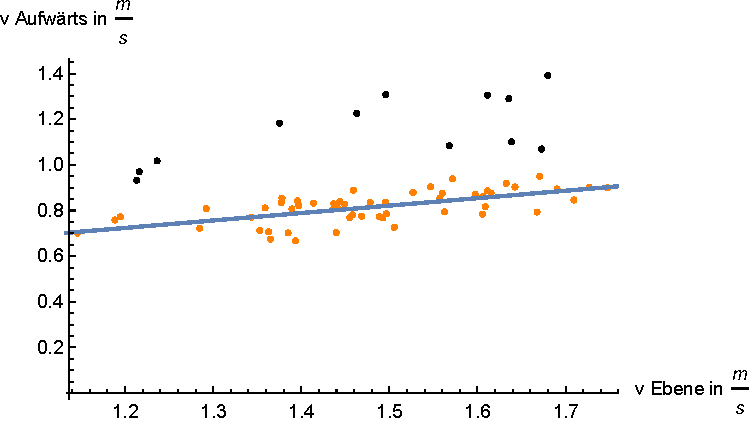
\includegraphics[]{abbildungen/regression/2017/ohneausreisser/auf-ebene.pdf}
	\[\begin{array}{l|llll}
 \text{} & \text{Estimate} & \text{Standard Error} & \text{t-Statistic} & \text{P-Value} \\
\hline
 1 & 0.506746 & 0.0900029 & 5.63033 & \text{2.603647901106944$\grave{ }$*${}^{\wedge}$-6} \\
 \text{vEbene} & 0.168071 & 0.0588553 & 2.85567 & 0.00727064 \\
\end{array}\]


	\caption{Abhängigkeit Wunschgeschwindigkeit in der Ebene zur Treppengeschwindigkeit aufwärts. Gefilterte Messdaten (orange) und Ausreißer (schwarz) mit ermittelter Regressionsgerade (blau). \label{fig:ohne-auf2017-ebene}}
\end{figure}

\begin{figure} \centering 
	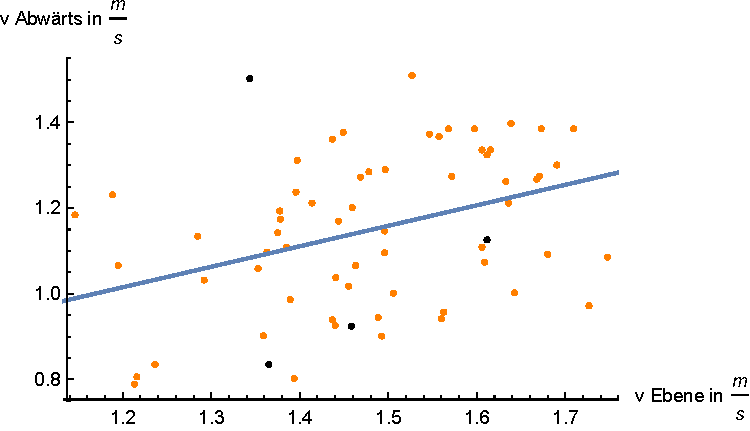
\includegraphics[]{abbildungen/regression/2017/ohneausreisser/ab-ebene.pdf}
	\[\begin{array}{l|llll}
 \text{} & \text{Estimate} & \text{Standard Error} & \text{t-Statistic} & \text{P-Value} \\
\hline
 1 & 0.440848 & 0.213068 & 2.06904 & 0.0428577 \\
 \text{vEbene} & 0.478525 & 0.142985 & 3.34668 & 0.00141579 \\
\end{array}\]


	\caption{Abhängigkeit Wunschgeschwindigkeit in der Ebene zur Treppengeschwindigkeit abwärts. Gefilterte Messdaten (orange) und Ausreißer (schwarz) mit ermittelter Regressionsgerade (blau).
	\label{fig:ohne-ab2017-ebene}}
\end{figure}

Für die Plausibilisierung der Regression wird die Nullhypothese 
$H_0: \beta_1 = 0$ aufgestellt. Signifikanzniveau $\alpha = 0.05$.
Die Ergebnisse des Tests sind in Abbildung \ref{fig:auf2017-ebene} zu sehen.
Signifikanz liegt vor, weil $p < \alpha$. Man verwirft die
Nullhypothese. Kein Einfluss von $v_{ebene}$ auf $v_{auf}$ wäre unplausibel, wenn auch nicht ausgeschlossen.

Die Nullhypothese und das Signifikanzniveau sind für alle folgenden Regressionen gleich. Die Ergebnisse für den Abstieg sind in Abbildung \ref{fig:ab2017-ebene} zu sehen.
Signifikanz liegt vor, weil $p < \alpha$. Man verwirft die
Nullhypothese. Kein Einfluss von $v_{ebene}$ auf $v_{ab}$ wäre unplausibel, wenn auch nicht ausgeschlossen.

\subsubsection{Körpergröße}

Für die Abhängigkeit Körpergröße wurde 
der Zusammenhang (\ref{eq:auf2017-groesse}) und (\ref{eq:ab2017-groesse}) ermittelt.

\begin{equation} \label{eq:auf2017-groesse}
	v_{auf}(groesse) = 0.133389 + 0.00419914 groesse
\end{equation}
\begin{equation} \label{eq:ab2017-groesse}
	v_{ab}(groesse) = 1.59558 - 0.00253145 groesse
\end{equation}

In den Abbildungen \ref{fig:auf2017-groesse} und \ref{fig:ab2017-groesse} ist 
zu sehen, dass nach dem Modell größere Personen leicht schneller Treppen besteigen, aber beim herabsteigen etwas langsamer als kleinere
Personen sind. 

\begin{figure} \centering 
	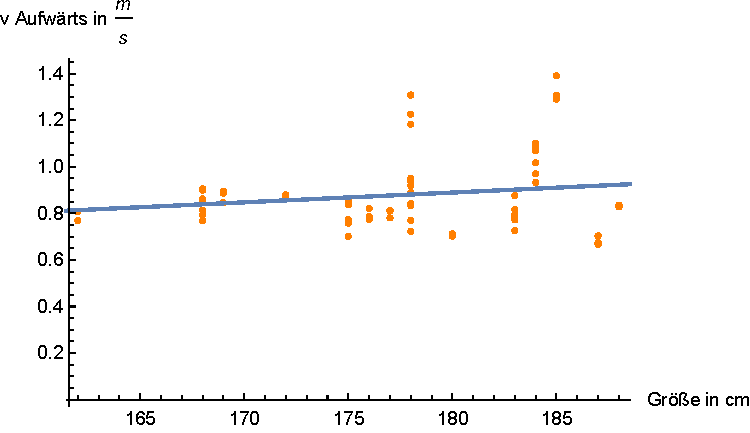
\includegraphics[]{abbildungen/regression/2017/auf-groesse.pdf}
	\[\begin{array}{l|llll}
 \text{} & \text{Estimate} & \text{Standard Error} & \text{t-Statistic} & \text{P-Value} \\
\hline
 1 & 1.42188 & 0.660147 & 2.15388 & 0.0335816 \\
 \text{gr{\" o}{\ss}e} & -0.00301832 & 0.0037105 & -0.813455 & 0.417834 \\
\end{array}\]


	\caption{Abhängigkeit Körpergröße zur Treppengeschwindigkeit aufwärts. Messdaten (orange) mit ermittelter Regressionsgerade (blau). \label{fig:auf2017-groesse}}
\end{figure}

\begin{figure} \centering 
	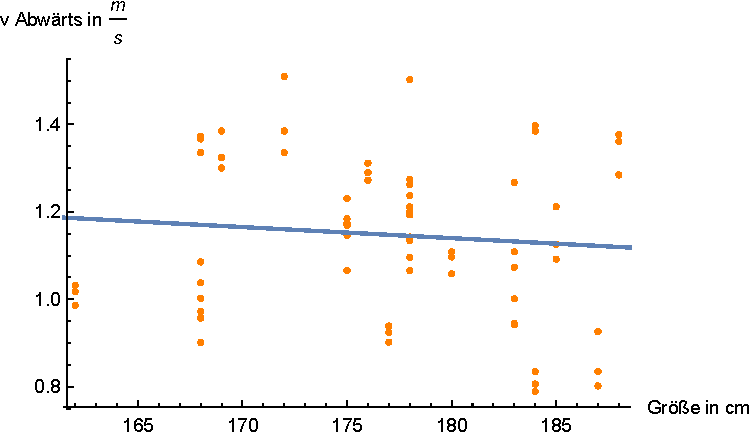
\includegraphics[]{abbildungen/regression/2017/ab-groesse.pdf}
	\[\begin{array}{l|llll}
 \text{} & \text{Estimate} & \text{Standard Error} & \text{t-Statistic} & \text{P-Value} \\
\hline
 1 & 1.59558 & 0.582855 & 2.73753 & 0.00800578 \\
 \text{gr{\" o}{\ss}e} & -0.00253145 & 0.00328881 & -0.769715 & 0.444301 \\
\end{array}\]


	\caption{Abhängigkeit Körpergröße zur Treppengeschwindigkeit abwärts. Messdaten (orange) mit ermittelter Regressionsgerade (blau). \label{fig:ab2017-groesse}}
\end{figure}

Ergebnisse der Plausibilisierung für den Aufstieg 
(Abbildung \ref{fig:auf2017-groesse}):
Signifikanz liegt nicht vor, weil $p > \alpha$. Man nimmt die
Nullhypothese an. Kein Einfluss von $groesse$ auf $v_{auf}$ ist plausibel.

Ergebnisse der Plausibilisierung für den Abstieg
(Abbildung \ref{fig:ab2017-groesse}):
Signifikanz liegt vor, weil $p > \alpha$. Man nimmt die
Nullhypothese an. Kein Einfluss von $groesse$ auf $v_{ab}$ ist plausibel.


\subsubsection{Rundennummer}


Für die Abhängigkeit Rundennummer wurde 
der Zusammenhang (\ref{eq:auf2017-runde}) und (\ref{eq:ab2017-runde}) ermittelt.

\begin{equation} \label{eq:auf2017-runde}
v_{auf}(runde) = 0.890435 - 0.00670795 runde
\end{equation}
\begin{equation} \label{eq:ab2017-runde}
v_{ab}(runde) = 1.14614\, +0.000574582 runde
\end{equation}

In den Abbildungen \ref{fig:auf2017-runde} und \ref{fig:ab2017-runde} ist 
zu sehen, dass sich nach dem Modell die Treppengeschwindigkeit bei Änderung der Runde fast nicht ändert. 

\begin{figure} \centering 
	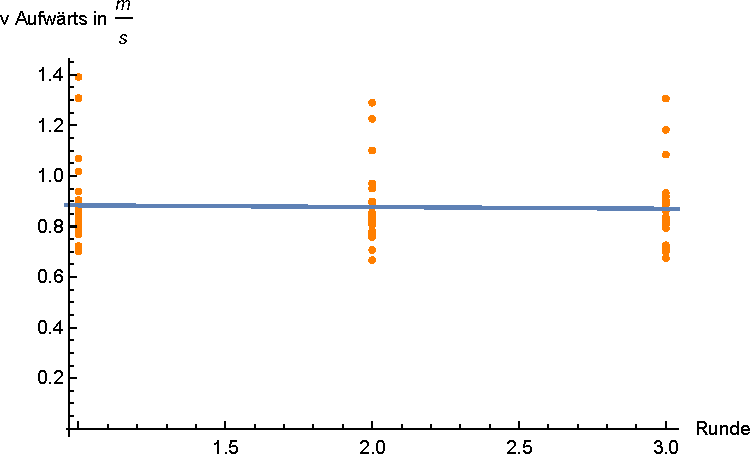
\includegraphics[]{abbildungen/regression/2017/auf-runde.pdf}
	\[\begin{array}{l|llll}
 \text{} & \text{Estimate} & \text{Standard Error} & \text{t-Statistic} & \text{P-Value} \\
\hline
 1 & 0.94804 & 0.2081 & 4.55569 & 0.0000551454 \\
 \text{runde} & -0.0241206 & 0.0963317 & -0.250391 & 0.80367 \\
\end{array}\]


	\caption{Abhängigkeit Rundennummer zur Treppengeschwindigkeit aufwärts. Messdaten (orange) mit ermittelter Regressionsgerade (blau). \label{fig:auf2017-runde}}
\end{figure}

\begin{figure} \centering 
	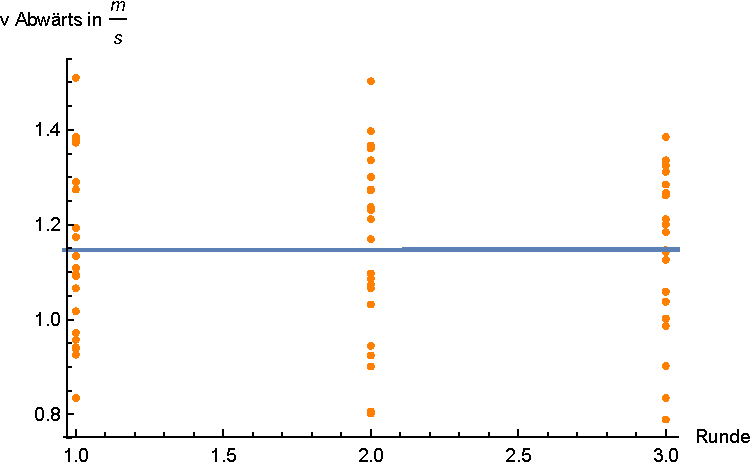
\includegraphics[]{abbildungen/regression/2017/ab-runde.pdf}
	\[\begin{array}{l|llll}
 \text{} & \text{Estimate} & \text{Standard Error} & \text{t-Statistic} & \text{P-Value} \\
\hline
 1 & 0.859522 & 0.0289618 & 29.6777 & \text{6.817362585804904$\grave{ }$*${}^{\wedge}$-26} \\
 \text{runde} & 0.00475595 & 0.0134067 & 0.354744 & 0.724973 \\
\end{array}\]


	\caption{Abhängigkeit Rundennummer zur Treppengeschwindigkeit abwärts. Messdaten (orange) mit ermittelter Regressionsgerade (blau). \label{fig:ab2017-runde}}
\end{figure}

Ergebnisse der Plausibilisierung für den Aufstieg
(Abbildung \ref{fig:auf2017-runde}):
Signifikanz liegt nicht vor, weil $p > \alpha$. Man nimmt die
Nullhypothese an. Kein Einfluss von $runde$ auf $v_{auf}$ ist plausibel.

Ergebnisse der Plausibilisierung für den Abstieg
(Abbildung \ref{fig:ab2017-runde}):
Signifikanz liegt vor, weil $p > \alpha$. Man nimmt die
Nullhypothese an. Kein Einfluss von $runde$ auf $v_{ab}$ ist plausibel.

\subsection{Mehrere Abhängigkeiten}

Hier werden weitere vier lineare Gleichungen mit mehreren Parametern ermittelt.

\[v_{auf}(v_{ebene}, groesse) = \beta_0 + \beta_1 v_{ebene} + \beta_2 groesse\]
\[v_{ab}(v_{ebene}, groesse) = \beta_0 + \beta_1 v_{ebene} + \beta_2 groesse\]

\[v_{auf}(v_{ebene}, groesse, runde) = \beta_0 + \beta_1 v_{ebene} + \beta_2 groesse + \beta_3 runde\]
\[v_{ab}(v_{ebene}, groesse, runde) = \beta_0 + \beta_1 v_{ebene} + \beta_2 groesse + \beta_3 runde\]

Für die Plausibilisierung der Regression wird die Nullhypothese 
$H_0: \beta_1 = 0  \lor \beta_2 = 0$ bzw. $H_0: \beta_1 = 0  \lor \beta_2 = 0 \lor \beta_3 = 0$ aufgestellt.

\subsubsection{Ebenengeschwindigkeit und Größe}

Für die Abhängigkeiten Wunschgeschwindigkeit in der Ebene und Körpergröße wurde 
der Zusammenhang (\ref{eq:auf2017-ebene-groesse}) und (\ref{eq:ab2017-ebene-groesse}) ermittelt.

\begin{equation} \label{eq:auf2017-ebene-groesse}
	v_{auf}(v_{ebene}, groesse) = -0.691667 + 0.425116 v_{ebene} + 0.00530344 groesse
\end{equation}
\begin{equation} \label{eq:ab2017-ebene-groesse}
	v_{auf}(v_{ebene}, groesse) = 0.731523 + 0.445214 v_{ebene} + -0.00137494 groesse
\end{equation}

In den Abbildungen \ref{fig:auf2017-ebene-groesse} und \ref{fig:ab2017-ebene-groesse} ist 
zu sehen, dass ein größerer Proband mit schnellerer Ebenengeschwindigkeit auch eine schnellere Treppengeschwindigkeit aufwärts erreicht. Eine schnellere Treppengeschwindigkeit abwärts wird durch einen Proband mit schnellerer Ebenengeschwindigkeit und kleinerer Größe erreicht. Eine Änderung von $50 cm$ in der Größe wirkt sich auf das Besteigen aufwärts mit ca. $0.25 m/s$ und abwärts mit ca. $0.05 m/s$ aus.

\begin{figure} \centering 
	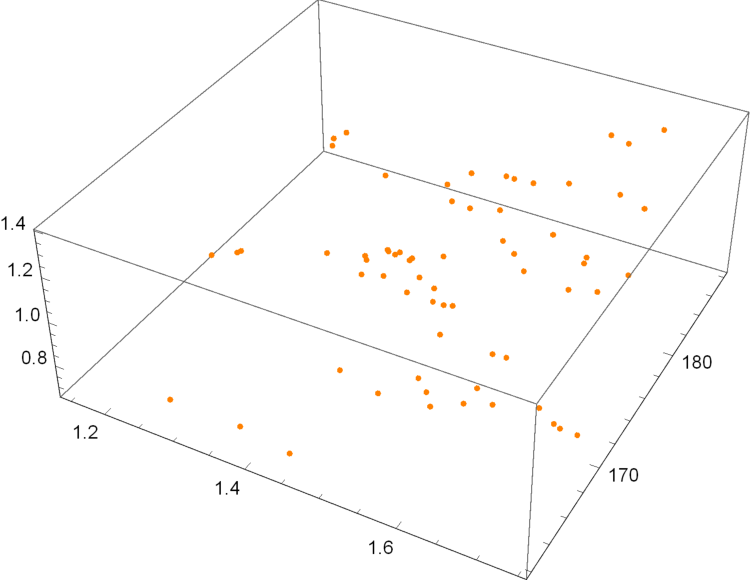
\includegraphics[]{abbildungen/regression/2017/auf-ebene-groesse.pdf}
	\[\begin{array}{l|llll}
 \text{} & \text{Estimate} & \text{Standard Error} & \text{t-Statistic} & \text{P-Value} \\
\hline
 1 & 1.0165 & 0.140132 & 7.25384 & \text{1.5820003769083974$\grave{ }$*${}^{\wedge}$-10} \\
 \text{vEbene} & 0.199894 & 0.0433176 & 4.61461 & 0.0000134806 \\
 \text{gr{\" o}{\ss}e} & -0.00294506 & 0.000643082 & -4.5796 & 0.0000154292 \\
\end{array}\]


	\caption{Abhängigkeiten Ebenengeschwindigkeit und Größe zur Treppengeschwindigkeit aufwärts. Messdaten (orange) mit ermittelter Regressionsebene (blau). \label{fig:auf2017-ebene-groesse}}
\end{figure}

\begin{figure} \centering 
	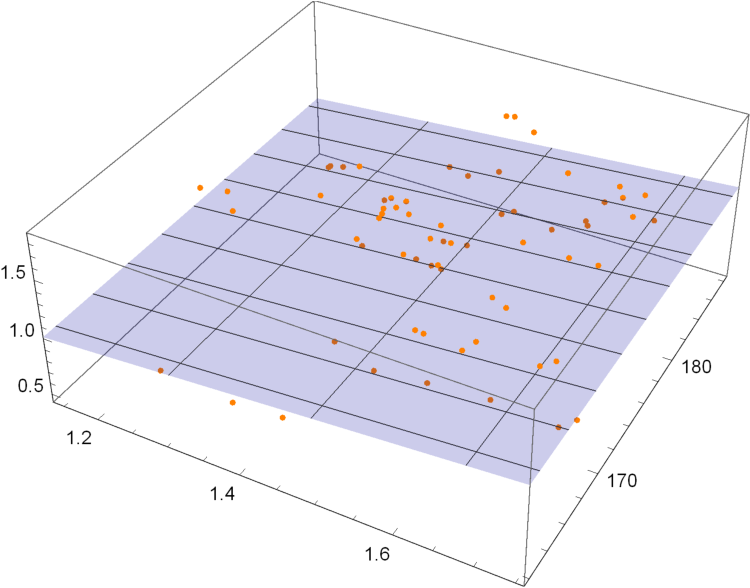
\includegraphics[]{abbildungen/regression/2017/ab-ebene-groesse.pdf}
	\[\begin{array}{l|llll}
 \text{} & \text{Estimate} & \text{Standard Error} & \text{t-Statistic} & \text{P-Value} \\
\hline
 1 & 0.701775 & 0.543236 & 1.29184 & 0.199331 \\
 \text{vEbene} & 0.696676 & 0.127843 & 5.44946 & \text{3.523565756565165$\grave{ }$*${}^{\wedge}$-7} \\
 \text{gr{\" o}{\ss}e} & -0.00382545 & 0.00268911 & -1.42257 & 0.157912 \\
\end{array}\]


	\caption{Abhängigkeiten Ebenengeschwindigkeit und Größe zur Treppengeschwindigkeit abwärts. Messdaten (orange) mit ermittelter Regressionsebene (blau). \label{fig:ab2017-ebene-groesse}}
\end{figure}

Ergebnisse der Plausibilisierung für den Aufstieg
(Abbildung \ref{fig:auf2017-ebene-groesse}):
Signifikanz liegt vor, weil beide $p < \alpha$. Man lehnt die
Nullhypothese ab. Kein Einfluss von $v_{ebene}$ und $groesse$ auf $v_{auf}$ ist unplausibel.

Ergebnisse der Plausibilisierung für den Abstieg
(Abbildung \ref{fig:ab2017-ebene-groesse}):
Signifikanz liegt nicht vor, weil $p_{\beta_2} > \alpha$. Man nimmt die
Nullhypothese an. Kein Einfluss von $v_{ebene}$ und $groesse$ auf $v_{ab}$ ist plausibel.


\subsubsection{Ebenengeschwindigkeit, Größe und Rundennummer}

Für die Abhängigkeiten Wunschgeschwindigkeit in der Ebene, Körpergröße und Rundennummer wurde 
der Zusammenhang (\ref{eq:auf2017-ebene-groesse-runde}) und (\ref{eq:ab2017-ebene-groesse-runde}) ermittelt.

\begin{multline} \label{eq:auf2017-ebene-groesse-runde}
v_{auf}(v_{ebene}, groesse, runde) = \\
-0.68569 + 0.424337 v_{ebene} + 0.00530141 groesse + -0.00223211 runde
\end{multline}
\begin{multline} \label{eq:ab2017-ebene-groesse-runde}
v_{auf}(v_{ebene}, groesse, runde) = \\
0.717358 + 0.447061 v_{ebene} + -0.00137015 groesse + 0.00529011 runde
\end{multline}

\begin{figure} \centering 
	\[\begin{array}{l|llll}
 \text{} & \text{Estimate} & \text{Standard Error} & \text{t-Statistic} & \text{P-Value} \\
\hline
 1 & 1.01208 & 0.137206 & 7.37634 & \text{2.1703587613814404$\grave{ }$*${}^{\wedge}$-8} \\
 \text{vEbene} & 0.117482 & 0.0493951 & 2.37842 & 0.0235248 \\
 \text{gr{\" o}{\ss}e} & -0.00231594 & 0.000542029 & -4.27274 & 0.000161828 \\
 \text{runde} & -0.00663057 & 0.00696761 & -0.951628 & 0.348419 \\
\end{array}\]


	\caption{Abhängigkeiten Ebenengeschwindigkeit, Größe und Runde zur Treppengeschwindigkeit aufwärts.
	\label{fig:auf2017-ebene-groesse-runde}}
\end{figure}

\begin{figure} \centering 
	\[\begin{array}{l|llll}
 \text{} & \text{Estimate} & \text{Standard Error} & \text{t-Statistic} & \text{P-Value} \\
\hline
 1 & 1.54231 & 0.231512 & 6.66191 & \text{1.6207125042011794$\grave{ }$*${}^{\wedge}$-7} \\
 \text{vEbene} & -0.070368 & 0.083346 & -0.844287 & 0.404777 \\
 \text{gr{\" o}{\ss}e} & -0.00320726 & 0.000914584 & -3.5068 & 0.00136734 \\
 \text{runde} & 0.0043198 & 0.0117567 & 0.367433 & 0.715715 \\
\end{array}\]


	\caption{Abhängigkeiten Ebenengeschwindigkeit, Größe und Runde zur Treppengeschwindigkeit abwärts.
	\label{fig:ab2017-ebene-groesse-runde}}
\end{figure}

Ergebnisse der Plausibilisierung für den Aufstieg
(Abbildung \ref{fig:auf2017-ebene-groesse-runde}):
Signifikanz liegt nicht vor, weil $p_{\beta_2} > \alpha$ und $p_{\beta_3} > \alpha$. Man nimmt die Nullhypothese an.

Ergebnisse der Plausibilisierung für den Abstieg
(Abbildung \ref{fig:ab2017-ebene-groesse-runde}):
Signifikanz liegt nicht vor, weil $p_{\beta_2} > \alpha$ und $p_{\beta_3} > \alpha$. Man nimmt die Nullhypothese an.

\subsection{Konditionierung}


\section{Ergebnisse}
\section{Ermitteltes Modell}

\section{Lineare Regression 2012}

Hier werden analog zu 2017 die Messdaten aus dem Experiment von 2012 mit linearer Regression betrachtet.

\subsection{Prüfung auf eine einfache Abhängigkeit}

Hier werden sechs Gleichungen mittels linearer Regression ermittelt: 

\[v_{auf}(v_{ebene}) = \beta_0 + \beta_1 v_{ebene}\]
\[v_{ab}(v_{ebene}) = \beta_0 + \beta_1 v_{ebene}\]

\[v_{auf}(groesse) = \beta_0 + \beta_1 groesse\]
\[v_{ab}(groesse) = \beta_0 + \beta_1 groesse\]

\[v_{auf}(runde) = \beta_0 + \beta_1 runde\]
\[v_{ab}(runde) = \beta_0 + \beta_1 runde\]

\subsubsection{Wunschgeschwindigkeit in der Ebene}

Für die Abhängigkeit Wunschgeschwindigkeit in der Ebene wurde 
der Zusammenhang wie in den Formeln für die Treppengeschwindigkeit aufwärts (\ref{eq:auf2012-ebene}) und abwärts (\ref{eq:ab2012-ebene}) ermittelt. 

\begin{equation} \label{eq:auf2012-ebene}
	v_{auf}(v_{ebene}) = -2.13306 + 1.92532 v_{ebene}
\end{equation}
\begin{equation} \label{eq:ab2012-ebene}
	v_{ab}(v_{ebene}) = -1.05942 + 1.28244 v_{ebene}
\end{equation}

Beide Steigungen sind positiv. Hat ein Proband eine schnellere Wunschgeschwindigkeit in der Ebene, verhält er sich auch schneller auf 
der Treppe. Die Abbildungen \ref{fig:auf2012-ebene} und \ref{fig:ab2012-ebene}
stellen dies grafisch dar. 

\begin{figure} \centering 
	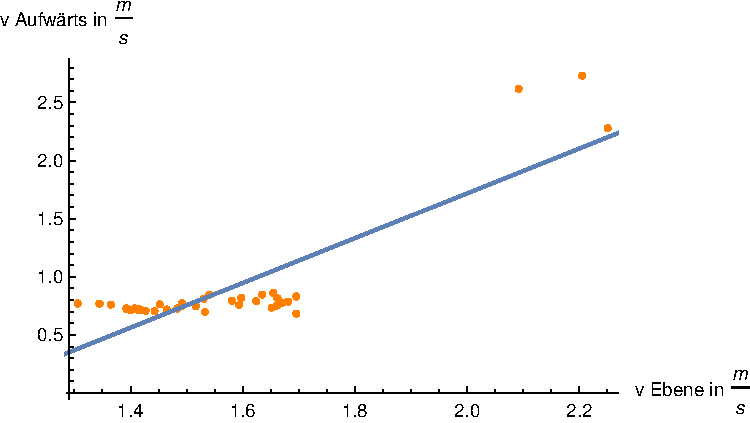
\includegraphics[]{abbildungen/regression/2012/auf-ebene.pdf}
	\[\begin{array}{l|llll}
 \text{} & \text{Estimate} & \text{Standard Error} & \text{t-Statistic} & \text{P-Value} \\
\hline
 1 & 0.506746 & 0.0900029 & 5.63033 & \text{2.603647901106944$\grave{ }$*${}^{\wedge}$-6} \\
 \text{vEbene} & 0.168071 & 0.0588553 & 2.85567 & 0.00727064 \\
\end{array}\]


	\caption{Abhängigkeit Wunschgeschwindigkeit in der Ebene zur Treppengeschwindigkeit aufwärts. Messdaten (orange) mit ermittelter Regressionsgerade (blau). \label{fig:auf2012-ebene}}
\end{figure}

\begin{figure} \centering 
	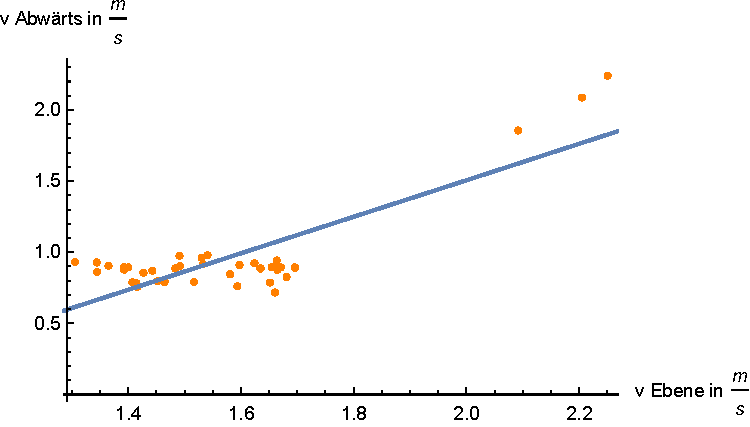
\includegraphics[]{abbildungen/regression/2012/ab-ebene.pdf}
	\[\begin{array}{l|llll}
 \text{} & \text{Estimate} & \text{Standard Error} & \text{t-Statistic} & \text{P-Value} \\
\hline
 1 & 0.440848 & 0.213068 & 2.06904 & 0.0428577 \\
 \text{vEbene} & 0.478525 & 0.142985 & 3.34668 & 0.00141579 \\
\end{array}\]


	\caption{Abhängigkeit Wunschgeschwindigkeit in der Ebene zur Treppengeschwindigkeit abwärts. Messdaten (orange) mit ermittelter Regressionsgerade (blau). \label{fig:ab2012-ebene}}
\end{figure}

In Abbildung \ref{fig:auf2012-ebene} sind wieder Ausreißer zu erkennen. In 2012 sind die Ausreißer (Datensätze mit Bemerkung) viel stärker ausgeprägt. Es ergeben sich neue Formeln für die Treppengeschwindigkeit aufwärts (\ref{eq:ohne-auf2012-ebene}) und abwärts (\ref{eq:ohne-ab2012-ebene}). Dazu gehören Abbildungen \ref{fig:ohne-auf2012-ebene} und \ref{fig:ohne-ab2012-ebene}.
Zur Vergleichbarkeit wurden aber dennoch in den weiteren Regressionen alle Daten (mit Ausreißern) verwendet.


\begin{equation} \label{eq:ohne-auf2012-ebene}
	v'_{auf}(v_{ebene}) = 0.506746 + 0.168071  v_{ebene}
\end{equation}
\begin{equation} \label{eq:ohne-ab2012-ebene}
	v'_{ab}(v_{ebene}) = 0.875577 - 0.00429171 v_{ebene}
\end{equation}

\begin{figure} \centering 
	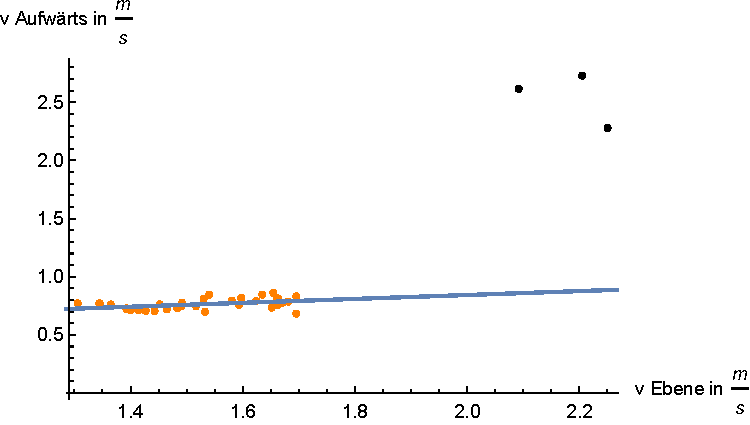
\includegraphics[]{abbildungen/regression/2012/ohneausreisser/auf-ebene.pdf}
	\[\begin{array}{l|llll}
 \text{} & \text{Estimate} & \text{Standard Error} & \text{t-Statistic} & \text{P-Value} \\
\hline
 1 & 0.506746 & 0.0900029 & 5.63033 & \text{2.603647901106944$\grave{ }$*${}^{\wedge}$-6} \\
 \text{vEbene} & 0.168071 & 0.0588553 & 2.85567 & 0.00727064 \\
\end{array}\]


	\caption{Abhängigkeit Wunschgeschwindigkeit in der Ebene zur Treppengeschwindigkeit aufwärts. Gefilterte Messdaten (orange) und Ausreißer (schwarz) mit ermittelter Regressionsgerade (blau). \label{fig:ohne-auf2012-ebene}}
\end{figure}

\begin{figure} \centering 
	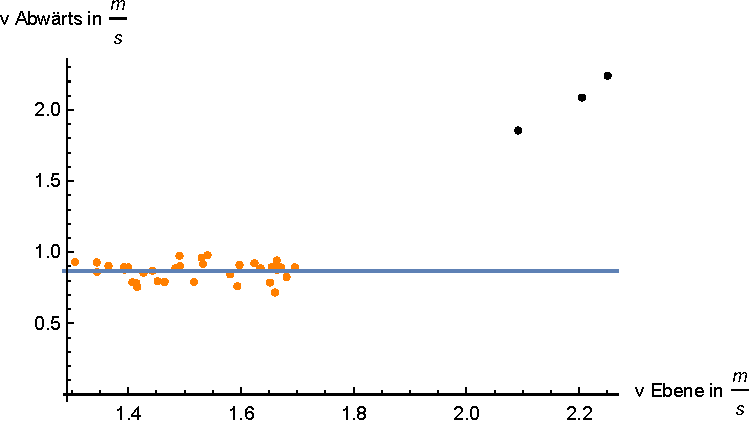
\includegraphics[]{abbildungen/regression/2012/ohneausreisser/ab-ebene.pdf}
	\[\begin{array}{l|llll}
 \text{} & \text{Estimate} & \text{Standard Error} & \text{t-Statistic} & \text{P-Value} \\
\hline
 1 & 0.440848 & 0.213068 & 2.06904 & 0.0428577 \\
 \text{vEbene} & 0.478525 & 0.142985 & 3.34668 & 0.00141579 \\
\end{array}\]


	\caption{Abhängigkeit Wunschgeschwindigkeit in der Ebene zur Treppengeschwindigkeit abwärts. Gefilterte Messdaten (orange) und Ausreißer (schwarz) mit ermittelter Regressionsgerade (blau).
	\label{fig:ohne-ab2012-ebene}}
\end{figure}

Für die Plausibilisierung der Regression wird die Nullhypothese 
$H_0: \beta_1 = 0$ aufgestellt. Signifikanzniveau $\alpha = 0.05$.
Die Ergebnisse des Tests sind in Abbildung \ref{fig:auf2012-ebene} zu sehen.
Signifikanz liegt vor, weil $p < \alpha$. Man verwirft die
Nullhypothese. Kein Einfluss von $v_{ebene}$ auf $v_{auf}$ wäre unplausibel, wenn auch nicht ausgeschlossen.

Die Nullhypothese und das Signifikanzniveau sind für alle folgenden Regressionen gleich. Die Ergebnisse für den Abstieg sind in Abbildung \ref{fig:ab2012-ebene} zu sehen.
Signifikanz liegt vor, weil $p < \alpha$. Man verwirft die
Nullhypothese. Kein Einfluss von $v_{ebene}$ auf $v_{ab}$ wäre unplausibel, wenn auch nicht ausgeschlossen.

\subsubsection{Körpergröße}

Für die Abhängigkeit Körpergröße wurde 
der Zusammenhang (\ref{eq:auf2012-groesse}) und (\ref{eq:ab2012-groesse}) ermittelt.

\begin{equation} \label{eq:auf2012-groesse}
	v_{auf}(groesse) = 2.428 - 0.00854845 groesse
\end{equation}
\begin{equation} \label{eq:ab2012-groesse}
	v_{ab}(groesse) = 2.20944 - 0.00698501 groesse
\end{equation}

In den Abbildungen \ref{fig:auf2012-groesse} und \ref{fig:ab2012-groesse} ist 
zu sehen, dass sich nach dem Modell größere Personen egal ob aufwärts oder abwärts langsamer auf der Treppe bewegen.

\begin{figure} \centering 
	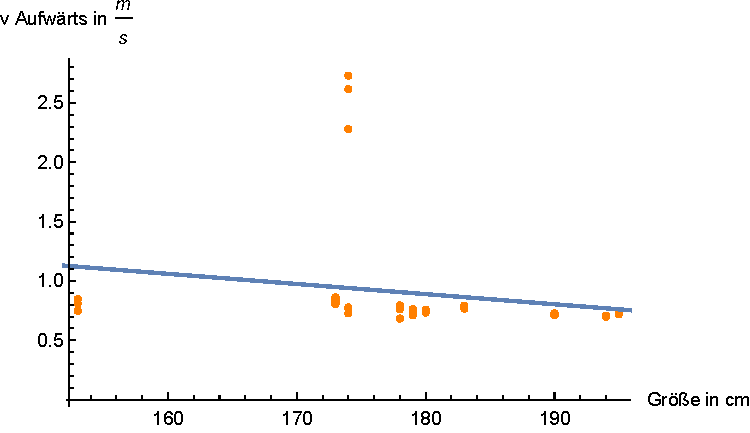
\includegraphics[]{abbildungen/regression/2012/auf-groesse.pdf}
	\[\begin{array}{l|llll}
 \text{} & \text{Estimate} & \text{Standard Error} & \text{t-Statistic} & \text{P-Value} \\
\hline
 1 & 1.42188 & 0.660147 & 2.15388 & 0.0335816 \\
 \text{gr{\" o}{\ss}e} & -0.00301832 & 0.0037105 & -0.813455 & 0.417834 \\
\end{array}\]


	\caption{Abhängigkeit Körpergröße zur Treppengeschwindigkeit aufwärts. Messdaten (orange) mit ermittelter Regressionsgerade (blau). \label{fig:auf2012-groesse}}
\end{figure}

\begin{figure} \centering 
	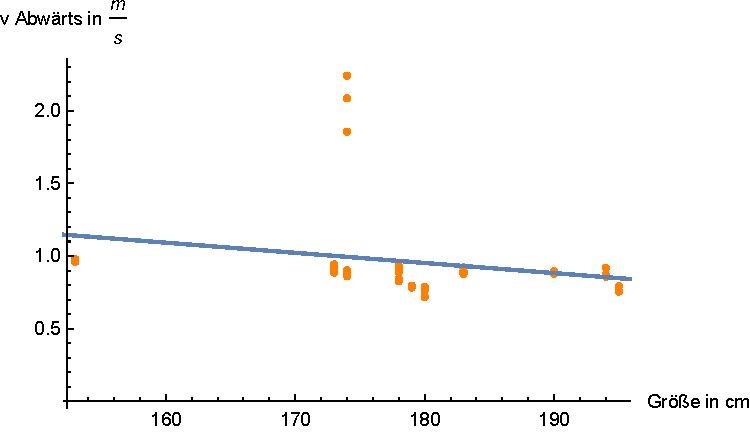
\includegraphics[]{abbildungen/regression/2012/ab-groesse.pdf}
	\[\begin{array}{l|llll}
 \text{} & \text{Estimate} & \text{Standard Error} & \text{t-Statistic} & \text{P-Value} \\
\hline
 1 & 1.59558 & 0.582855 & 2.73753 & 0.00800578 \\
 \text{gr{\" o}{\ss}e} & -0.00253145 & 0.00328881 & -0.769715 & 0.444301 \\
\end{array}\]


	\caption{Abhängigkeit Körpergröße zur Treppengeschwindigkeit abwärts. Messdaten (orange) mit ermittelter Regressionsgerade (blau). \label{fig:ab2012-groesse}}
\end{figure}

Ergebnisse der Plausibilisierung für den Aufstieg 
(Abbildung \ref{fig:auf2012-groesse}):
Signifikanz liegt nicht vor, weil $p > \alpha$. Man nimmt die
Nullhypothese an. Kein Einfluss von $groesse$ auf $v_{auf}$ ist plausibel.

Ergebnisse der Plausibilisierung für den Abstieg
(Abbildung \ref{fig:ab2012-groesse}):
Signifikanz liegt vor, weil $p > \alpha$. Man nimmt die
Nullhypothese an. Kein Einfluss von $groesse$ auf $v_{ab}$ ist plausibel.


\subsubsection{Rundennummer}


Für die Abhängigkeit Rundennummer wurde 
der Zusammenhang (\ref{eq:auf2012-runde}) und (\ref{eq:ab2012-runde}) ermittelt.

\begin{equation} \label{eq:auf2012-runde}
v_{auf}(runde) = 0.940079 - 0.0241206 runde
\end{equation}
\begin{equation} \label{eq:ab2012-runde}
v_{ab}(runde) = 0.940079 + 0.0103279 runde
\end{equation}

In den Abbildungen \ref{fig:auf2012-runde} und \ref{fig:ab2012-runde} ist 
zu sehen, dass sich nach dem Modell die Treppengeschwindigkeit bei Änderung der Runde fast nicht ändert. 

\begin{figure} \centering 
	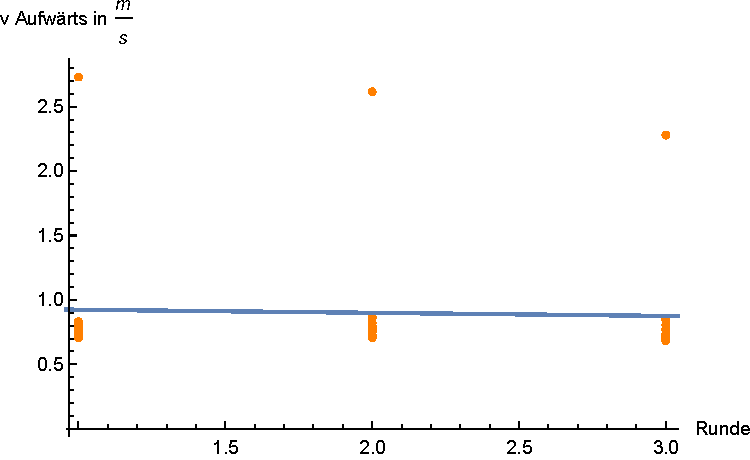
\includegraphics[]{abbildungen/regression/2012/auf-runde.pdf}
	\[\begin{array}{l|llll}
 \text{} & \text{Estimate} & \text{Standard Error} & \text{t-Statistic} & \text{P-Value} \\
\hline
 1 & 0.94804 & 0.2081 & 4.55569 & 0.0000551454 \\
 \text{runde} & -0.0241206 & 0.0963317 & -0.250391 & 0.80367 \\
\end{array}\]


	\caption{Abhängigkeit Rundennummer zur Treppengeschwindigkeit aufwärts. Messdaten (orange) mit ermittelter Regressionsgerade (blau). \label{fig:auf2012-runde}}
\end{figure}

\begin{figure} \centering 
	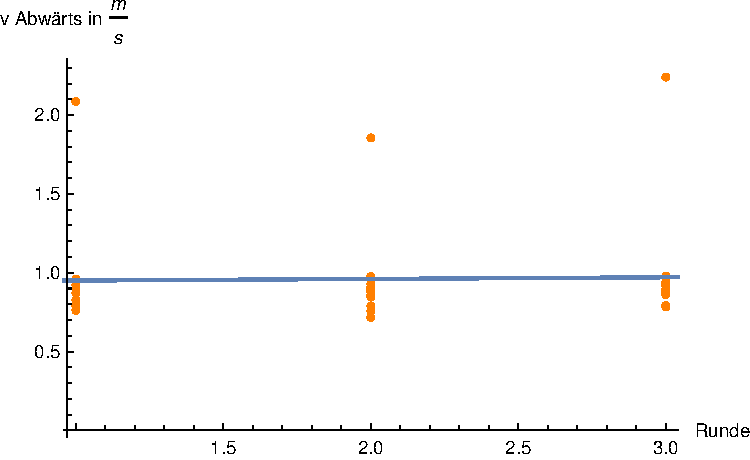
\includegraphics[]{abbildungen/regression/2012/ab-runde.pdf}
	\[\begin{array}{l|llll}
 \text{} & \text{Estimate} & \text{Standard Error} & \text{t-Statistic} & \text{P-Value} \\
\hline
 1 & 0.859522 & 0.0289618 & 29.6777 & \text{6.817362585804904$\grave{ }$*${}^{\wedge}$-26} \\
 \text{runde} & 0.00475595 & 0.0134067 & 0.354744 & 0.724973 \\
\end{array}\]


	\caption{Abhängigkeit Rundennummer zur Treppengeschwindigkeit abwärts. Messdaten (orange) mit ermittelter Regressionsgerade (blau). \label{fig:ab2012-runde}}
\end{figure}

Ergebnisse der Plausibilisierung für den Aufstieg
(Abbildung \ref{fig:auf2012-runde}):
Signifikanz liegt nicht vor, weil $p > \alpha$. Man nimmt die
Nullhypothese an. Kein Einfluss von $runde$ auf $v_{auf}$ ist plausibel.

Ergebnisse der Plausibilisierung für den Abstieg
(Abbildung \ref{fig:ab2012-runde}):
Signifikanz liegt vor, weil $p > \alpha$. Man nimmt die
Nullhypothese an. Kein Einfluss von $runde$ auf $v_{ab}$ ist plausibel.

\subsection{Mehrere Abhängigkeiten}

Hier werden weitere vier lineare Gleichungen mit mehreren Parametern ermittelt.

\[v_{auf}(v_{ebene}, groesse) = \beta_0 + \beta_1 v_{ebene} + \beta_2 groesse\]
\[v_{ab}(v_{ebene}, groesse) = \beta_0 + \beta_1 v_{ebene} + \beta_2 groesse\]

\[v_{auf}(v_{ebene}, groesse, runde) = \beta_0 + \beta_1 v_{ebene} + \beta_2 groesse + \beta_3 runde\]
\[v_{ab}(v_{ebene}, groesse, runde) = \beta_0 + \beta_1 v_{ebene} + \beta_2 groesse + \beta_3 runde\]

Für die Plausibilisierung der Regression wird die Nullhypothese 
$H_0: \beta_1 = 0  \lor \beta_2 = 0$ bzw. $H_0: \beta_1 = 0  \lor \beta_2 = 0 \lor \beta_3 = 0$ aufgestellt.

\subsubsection{Ebenengeschwindigkeit und Größe}

Für die Abhängigkeiten Wunschgeschwindigkeit in der Ebene und Körpergröße wurde 
der Zusammenhang (\ref{eq:auf2012-ebene-groesse}) und (\ref{eq:ab2012-ebene-groesse}) ermittelt.

\begin{equation} \label{eq:auf2012-ebene-groesse}
	v_{auf}(v_{ebene}, groesse) = -2.23812 7 + 1.93153 v_{ebene} + 0.000532946 groesse
\end{equation}
\begin{equation} \label{eq:ab2012-ebene-groesse}
	v_{auf}(v_{ebene}, groesse) = -0.860154 + 1.27065 v_{ebene} + -0.00101083 groesse
\end{equation}

In den Abbildungen \ref{fig:auf2012-ebene-groesse} und \ref{fig:ab2012-ebene-groesse} ist 
zu sehen, dass ein größerer Proband mit schnellerer Ebenengeschwindigkeit auch eine schnellere Treppengeschwindigkeit aufwärts erreicht. Eine schnellere Treppengeschwindigkeit abwärts wird durch einen Proband mit schnellerer Ebenengeschwindigkeit und kleinerer Größe erreicht. Eine Änderung von $50 cm$ in der Größe wirkt sich auf das Besteigen aufwärts mit ca. $0.025 m/s$ und abwärts mit ca. $0.05 m/s$ aus.

\begin{figure} \centering 
	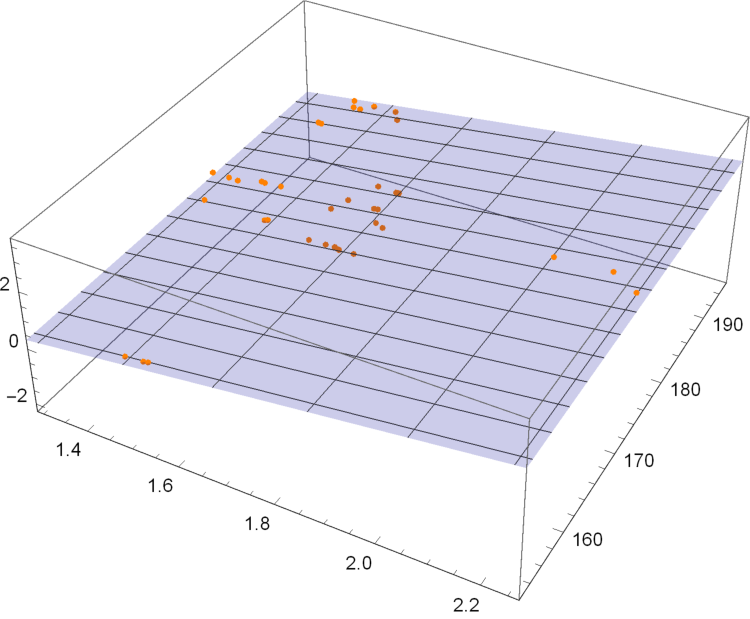
\includegraphics[]{abbildungen/regression/2012/auf-ebene-groesse.pdf}
	\[\begin{array}{l|llll}
 \text{} & \text{Estimate} & \text{Standard Error} & \text{t-Statistic} & \text{P-Value} \\
\hline
 1 & 1.0165 & 0.140132 & 7.25384 & \text{1.5820003769083974$\grave{ }$*${}^{\wedge}$-10} \\
 \text{vEbene} & 0.199894 & 0.0433176 & 4.61461 & 0.0000134806 \\
 \text{gr{\" o}{\ss}e} & -0.00294506 & 0.000643082 & -4.5796 & 0.0000154292 \\
\end{array}\]


	\caption{Abhängigkeiten Ebenengeschwindigkeit und Größe zur Treppengeschwindigkeit aufwärts. Messdaten (orange) mit ermittelter Regressionsebene (blau). \label{fig:auf2012-ebene-groesse}}
\end{figure}

\begin{figure} \centering 
	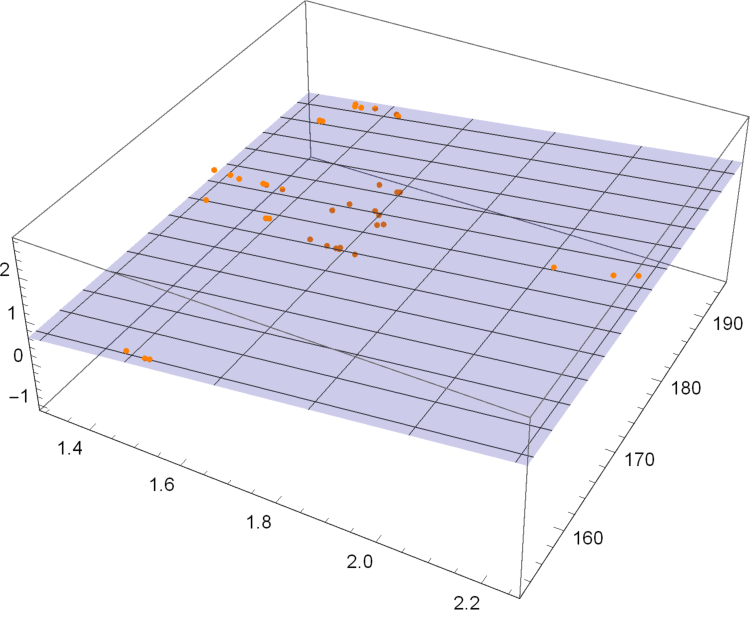
\includegraphics[]{abbildungen/regression/2012/ab-ebene-groesse.pdf}
	\[\begin{array}{l|llll}
 \text{} & \text{Estimate} & \text{Standard Error} & \text{t-Statistic} & \text{P-Value} \\
\hline
 1 & 0.701775 & 0.543236 & 1.29184 & 0.199331 \\
 \text{vEbene} & 0.696676 & 0.127843 & 5.44946 & \text{3.523565756565165$\grave{ }$*${}^{\wedge}$-7} \\
 \text{gr{\" o}{\ss}e} & -0.00382545 & 0.00268911 & -1.42257 & 0.157912 \\
\end{array}\]


	\caption{Abhängigkeiten Ebenengeschwindigkeit und Größe zur Treppengeschwindigkeit abwärts. Messdaten (orange) mit ermittelter Regressionsebene (blau). \label{fig:ab2012-ebene-groesse}}
\end{figure}

Ergebnisse der Plausibilisierung für den Aufstieg
(Abbildung \ref{fig:auf2012-ebene-groesse}):
Signifikanz liegt nicht vor, weil $p_{\beta_2} > \alpha$. Man nimmt die
Nullhypothese an. Kein Einfluss von $v_{ebene}$ und $groesse$ auf $v_{auf}$ ist plausibel.

Ergebnisse der Plausibilisierung für den Abstieg
(Abbildung \ref{fig:ab2012-ebene-groesse}):
Signifikanz liegt nicht vor, weil $p_{\beta_2} > \alpha$. Man nimmt die
Nullhypothese an. Kein Einfluss von $v_{ebene}$ und $groesse$ auf $v_{ab}$ ist plausibel.


\subsubsection{Ebenengeschwindigkeit, Größe und Rundennummer}

Für die Abhängigkeiten Wunschgeschwindigkeit in der Ebene, Körpergröße und Rundennummer wurde 
der Zusammenhang (\ref{eq:auf2012-ebene-groesse-runde}) und (\ref{eq:ab2012-ebene-groesse-runde}) ermittelt.

\begin{multline} \label{eq:auf2012-ebene-groesse-runde}
v_{auf}(v_{ebene}, groesse, runde) = \\
-2.20269 + 1.93049 v_{ebene} + 0.000528021 groesse - 0.0164501  runde
\end{multline}
\begin{multline} \label{eq:ab2012-ebene-groesse-runde}
v_{auf}(v_{ebene}, groesse, runde) = \\
- 0.893281 + 1.27163 v_{ebene} - 0.00100623 groesse + 0.0153806  runde
\end{multline}

\begin{figure} \centering 
	\[\begin{array}{l|llll}
 \text{} & \text{Estimate} & \text{Standard Error} & \text{t-Statistic} & \text{P-Value} \\
\hline
 1 & 1.01208 & 0.137206 & 7.37634 & \text{2.1703587613814404$\grave{ }$*${}^{\wedge}$-8} \\
 \text{vEbene} & 0.117482 & 0.0493951 & 2.37842 & 0.0235248 \\
 \text{gr{\" o}{\ss}e} & -0.00231594 & 0.000542029 & -4.27274 & 0.000161828 \\
 \text{runde} & -0.00663057 & 0.00696761 & -0.951628 & 0.348419 \\
\end{array}\]


	\caption{Abhängigkeiten Ebenengeschwindigkeit, Größe und Runde zur Treppengeschwindigkeit aufwärts.
	\label{fig:auf2012-ebene-groesse-runde}}
\end{figure}

\begin{figure} \centering 
	\[\begin{array}{l|llll}
 \text{} & \text{Estimate} & \text{Standard Error} & \text{t-Statistic} & \text{P-Value} \\
\hline
 1 & 1.54231 & 0.231512 & 6.66191 & \text{1.6207125042011794$\grave{ }$*${}^{\wedge}$-7} \\
 \text{vEbene} & -0.070368 & 0.083346 & -0.844287 & 0.404777 \\
 \text{gr{\" o}{\ss}e} & -0.00320726 & 0.000914584 & -3.5068 & 0.00136734 \\
 \text{runde} & 0.0043198 & 0.0117567 & 0.367433 & 0.715715 \\
\end{array}\]


	\caption{Abhängigkeiten Ebenengeschwindigkeit, Größe und Runde zur Treppengeschwindigkeit abwärts.
	\label{fig:ab2012-ebene-groesse-runde}}
\end{figure}

Ergebnisse der Plausibilisierung für den Aufstieg
(Abbildung \ref{fig:auf2012-ebene-groesse-runde}):
Signifikanz liegt nicht vor, weil $p_{\beta_2} > \alpha$ und $p_{\beta_3} > \alpha$. Man nimmt die Nullhypothese an.

Ergebnisse der Plausibilisierung für den Abstieg
(Abbildung \ref{fig:ab2012-ebene-groesse-runde}):
Signifikanz liegt nicht vor, weil $p_{\beta_2} > \alpha$ und $p_{\beta_3} > \alpha$. Man nimmt die Nullhypothese an.

\subsection{Vergleich mit Daten aus 2017}

Vergleicht man die Ergebnisse der Plausibilisierungen der Regressionen fällt sofort auf, das grundsätzlich für beide Jahre nur die Abhängigkeit zur freien Wunschgeschwindigkeit in der Ebene als plausibel bestimmt wurde (siehe Abbildung \ref{fig:plausibilisierung-2017-2012}). Nur das Modell für die Aufwärtsgeschwindigkeit berechnet durch Ebenengeschwindigkeit und Größe ist zusätzlich im Jahr 2017 plausibel. Diese Übereinstimmung ist auch zu erwarten, da ja beide Messexperimente gleich spezifiziert waren.

Der Unterschied im Modell mit der Größe ist durch das Eintreten eines Fehlers bei einem der beiden Hypothesentests, die Ausreißer, zu geringe Datenmenge oder sogar Unterschiede beider Experimente zu erklären.

Für die nicht sofort widerlegten Modelle basierend nur auf der Ebenengeschwindigkeit ist noch von Interesse, ob die Koeffizienten ähnlich sind. In Abbildung \ref{fig:steigung-2017-2012} ist zu sehen, dass die Steigungen zwar beide positiv sind, aber die 
Stärke unterschiedlich ist. Dies ist auf die extremen Ausreißer im Jahr 2012 zurückzuführen.


\begin{figure}
\[\begin{array}{cc l}
	\hline
	 2017 & 2012 & \text{Modell} \\
	\hline
	\checkmark&\checkmark& v_{auf}(v_{ebene}) \\
	\checkmark&\checkmark& v_{ab}(v_{ebene})\\
	
	&& v_{auf}(groesse) \\
	&& v_{ab}(groesse)  \\
	
	&& v_{auf}(runde) \\
	&& v_{ab}(runde)  \\	
	
	\checkmark&& v_{auf}(v_{ebene}, groesse) \\
	&& v_{ab}(v_{ebene}, groesse)  \\
		
	&& v_{auf}(v_{ebene}, groesse, runde)  \\
	&& v_{ab}(v_{ebene}, groesse, runde) \\	
	\hline
\end{array}\]
\caption{Liste aller betrachteten Regressionsmodelle und ob sie für den Datensatz aus dem jeweiligen Jahr plausibel sind.} \label{fig:plausibilisierung-2017-2012}
\end{figure}


\begin{figure}
	\[\begin{array}{r | cc}
	\hline
	 & \text{2017} & \text{2012} \\
	\hline
	v_{auf} & 0.393467 v_{ebene}& 1.92532 v_{ebene}  \\
	v_{ab} & 0.453419 v_{ebene}&1.28244 v_{ebene}  \\
	\hline
	\end{array}\]
	\caption{Steigung für die Ebenengeschwindigkeit aus den beiden Modellen von 2017 und 2012.} \label{fig:steigung-2017-2012}
\end{figure}



\section{Verbund von alten und neuen Daten}

\section{Fazit}

\end{document}
